\documentclass[reprint, nofootinbib, nobalancelastpage, 10pt]{revtex4-2}

\usepackage[T2A]{fontenc}			% кодировка
\usepackage[utf8]{inputenc}			% кодировка исходного текста
\usepackage[english,russian]{babel}	% локализация и переносы

\usepackage{amsmath,amsfonts,amssymb,amsthm,mathtools}

\usepackage[usenames]{color}
\usepackage{colortbl}
\usepackage{indentfirst} %Красная строка
\usepackage{hyperref}

\usepackage{booktabs}
\usepackage{graphicx}  % Для вставки рисунков
\graphicspath{{images/}{graphs/}}  % папки с картинками

\renewcommand*{\thefootnote}{\alph{footnote}}

\begin{document}

\title{Исследование поглощения вторичного космического излучения в веществе}
\author{Илларионов Владислав}
\affiliation{группа Б04-855}

\maketitle


\section*{Введение}

В результате взаимодействия протонов первичного излучения с ядрами атомов воздуха в
атмосфере Земли происходит расщепление ядер и рождение $\pi^{\pm}$-мезонов и
$\pi^0$-мезонов. Распад заряженных $\pi^{\pm}$-мезонов приводит к образованию жесткой
компоненты вторичного космического излучения, а распад нейтральных пионов $\pi^0$~--~к
образованию мягкой (электронно-фотонной) компоненты.

В данной работе по измерениям зависимости интенсивности космического излучения в
лаборатории от толщины поглотителя (пластины свинца) определяются эффективные длины
поглощения мягкой и жесткой компонент космики, а также абсолютные значения их вертикальных
интенсивностей.


\section*{Теоретическая часть}

Космические лучи~--~поток частиц высокой энергии, преимущественно протонов, приходящих
на Землю из мирового пространства (первичное излучение), а также рожденное ими в атмосфере
Земли из-за взаимодействия с атомными ядрами вторичное излучение. Результатом этого
взаимодействия преимущественно происходит рождение пионов, распад которых приводит к
образованию мюонов и гамма-квантов:

\begin{eqnarray*}
	\pi^+ &&\rightarrow \mu^+ + \nu_{\mu} \\
	\pi^- &&\rightarrow \mu^- + \widetilde{\nu}_{\mu} \\
	\pi^0 &&\rightarrow \gamma + \gamma
\end{eqnarray*}

Жесткая компонента в основном состоит из мюонов, которые не участвуют в ядерных (сильных)
взаимодействиях и практически не теряют своей энергии за счет тормозного излучения. Их
энергия тратится только на ионизацию вещества. Ионизационные потери релятивистских мюонов
слабо зависят от состава вещества и фактически определяются лишь поверхностной плотностью
поглотителя.

В отличие от мюонов, потеря энергии высокоэнергичными фотонами обусловлена процессом
рождения пар в веществе, а электроны теряют свою энергию за счет тормозного излучения.
Образовавшиеся фотоны с большой вероятностью снова рождают электрон-позитронные пары.
Так, быстро образуется лавина. С увеличением толщины поглотителя, все больше выбывает
электронов и позитронов, в следствие чего уменьшается количество регистрируемых частиц. 

Зависимость числа импульсов за определенный промежуток времени от толщины поглотителя $L$
можно описать функцией:

\begin{equation}
	\label{eq:expon}
	N = N_0 \exp \left(-\dfrac{\rho L}{\lambda} \right) + C
\end{equation}

\section*{Экспериментальная установка}

Основой измерительной установки является телескоп, ориентированный вертикально.Телескоп
состоит из нескольких рядов параллельно включенных счетчиков Гейгера-Мюллера. Он позволяет
регистрировать только частицы, пролетевшие через все счетчики, что достигается с помощью
схемы совпадений, посылающей в этом случае импульс напряжения на пересчетную схему.
Схема подает сигнал только если в малый промежуток времени $\tau \approx 10^{-7}$
сработают оба датчика.

Блок управления и индикации установки содержит:

\begin{enumerate}
	\item Таймер с максимальным временем измерения 999 с.
	\item Высоковольтный выпрямитель для питания счетчиков.
	\item Схему совпадений.
	\item Блок пересчета импульсов.
\end{enumerate}

Между детекторами можно вставлять различное количество свинцовых пластин. Длина пластин
$a = 30 \pm 0.05$ см, а их ширина $b = 8.4 \pm 0.05$ см. Расстояние между детекторами
составляет $l = 39 \pm 1$ см.

\section*{Методика измерения}

Количество частиц $N$, регистрируемых счетчиком, как дискретная случайная величина, может
быть описана распределением Пуассона ($\lambda = N$). Тогда относительная погрешность
определения $N$ будет равна:

\[ \varepsilon = \dfrac{\sqrt{N}}{N} = \dfrac{1}{\sqrt{N}} \]

Производится серия измерений зависимости количества регистрируемых импульсов от толщины
поглотителя за определенное время. Замеры ведутся одновременно на двух установках, после
чего производится анализ полученных данных. Для каждого значения толщины поглотителя
берется среднее значение количества импульсов в секунду.

По полученным данным аппроксимируем убывание количества частиц жесткой компоненты прямой
линией, после чего вычитаем из общего количества частиц значения аппроксимирующей прямой.
Так, получим количество частиц для мягкой компоненты вторичного излучения.

Также проводим аппроксимацию общего количества частиц и полученных ранее значений мягкой
компоненты экспоненциальной функцией вида:

\[ f(x) = A \exp \left(-\frac{x}{B} \right) + C,\text{\hspace*{20pt} A,B,C = const} \]

Тогда из формулы~(\ref{eq:expon}) можем найти длину свободного пробега как:
$\lambda = \rho B$, где $\rho$~--~плотность поглотителя (свинца).

Для подсчета длины свободного пробега жесткой компоненты вычтем из общего числа частиц
значение аппроксимации мягкой компоненты и снова аппроксимируем полученные значения все
той же экспоненциальной функцией.

Телесный угол, охватываемый телескопом будем вычислять, как:

\[ \Omega = \dfrac{4S}{l^2}, \]

где $S = ab$,~--~площадь пластины поглотителя. Телесный угол используется для расчета
интенсивностей мягкой и жесткой компонент.


\section*{Обработка данных}

В связи с ограниченностью времени, отведенного на эксперимент, установим время одного
измерения на 720 секунд. Также заметим, что при регистрации более 100 частиц,
статистическая погрешность будет менее 10\%.

Проведем серию измерений на двух установках, экспериментальные данные занесем в
таблицы~\ref{tab:data1}-\ref{tab:data2}. На основе полученных данных построим график
зависимости количества частиц в единицу времени от толщины поглотителя
(рис.~\ref{graph:gnrl}).

\begin{figure}[h!]
	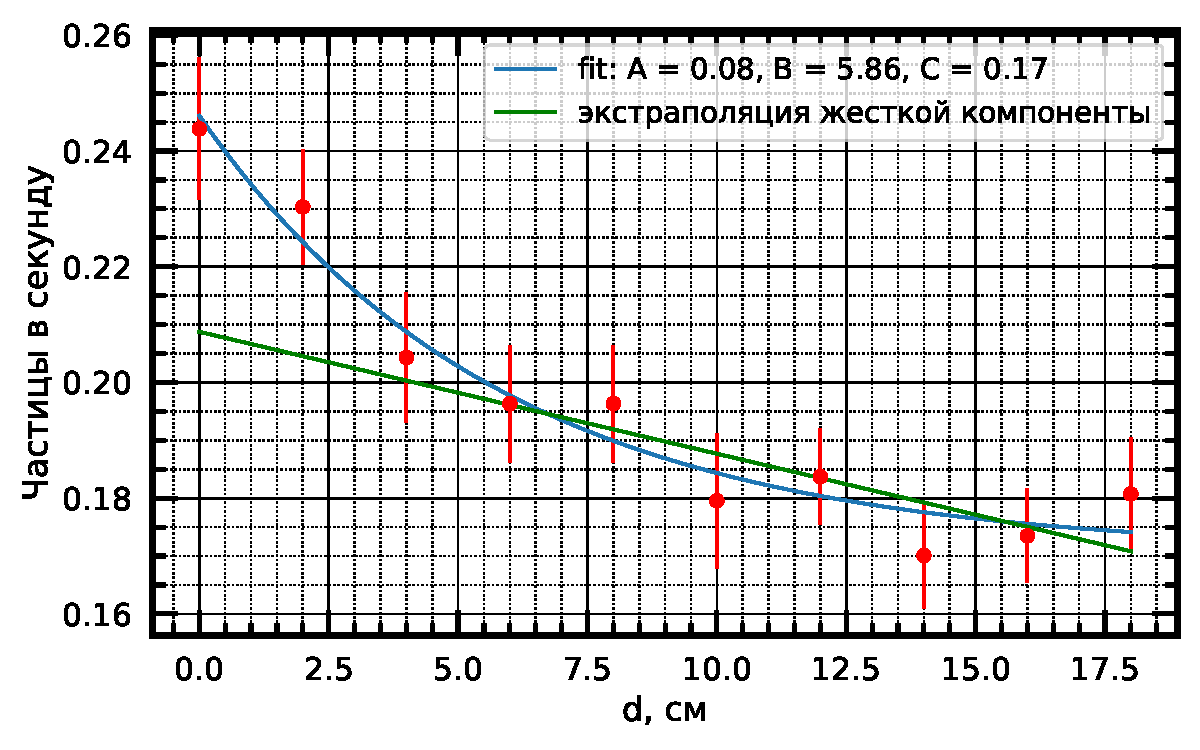
\includegraphics[width=0.95\linewidth]{plot_1.pdf}
	\caption{Зависимость количества регистрируемых частиц от толщины поглотителя}
	\label{graph:gnrl}
\end{figure}

Далее построим графики для мягкой компоненты (рис.~\ref{graph:soft}) и жесткой
(рис.~\ref{graph:hard}). Из аппроксимации рассчитаем длины свободного пробега:

\begin{figure}[h!]
	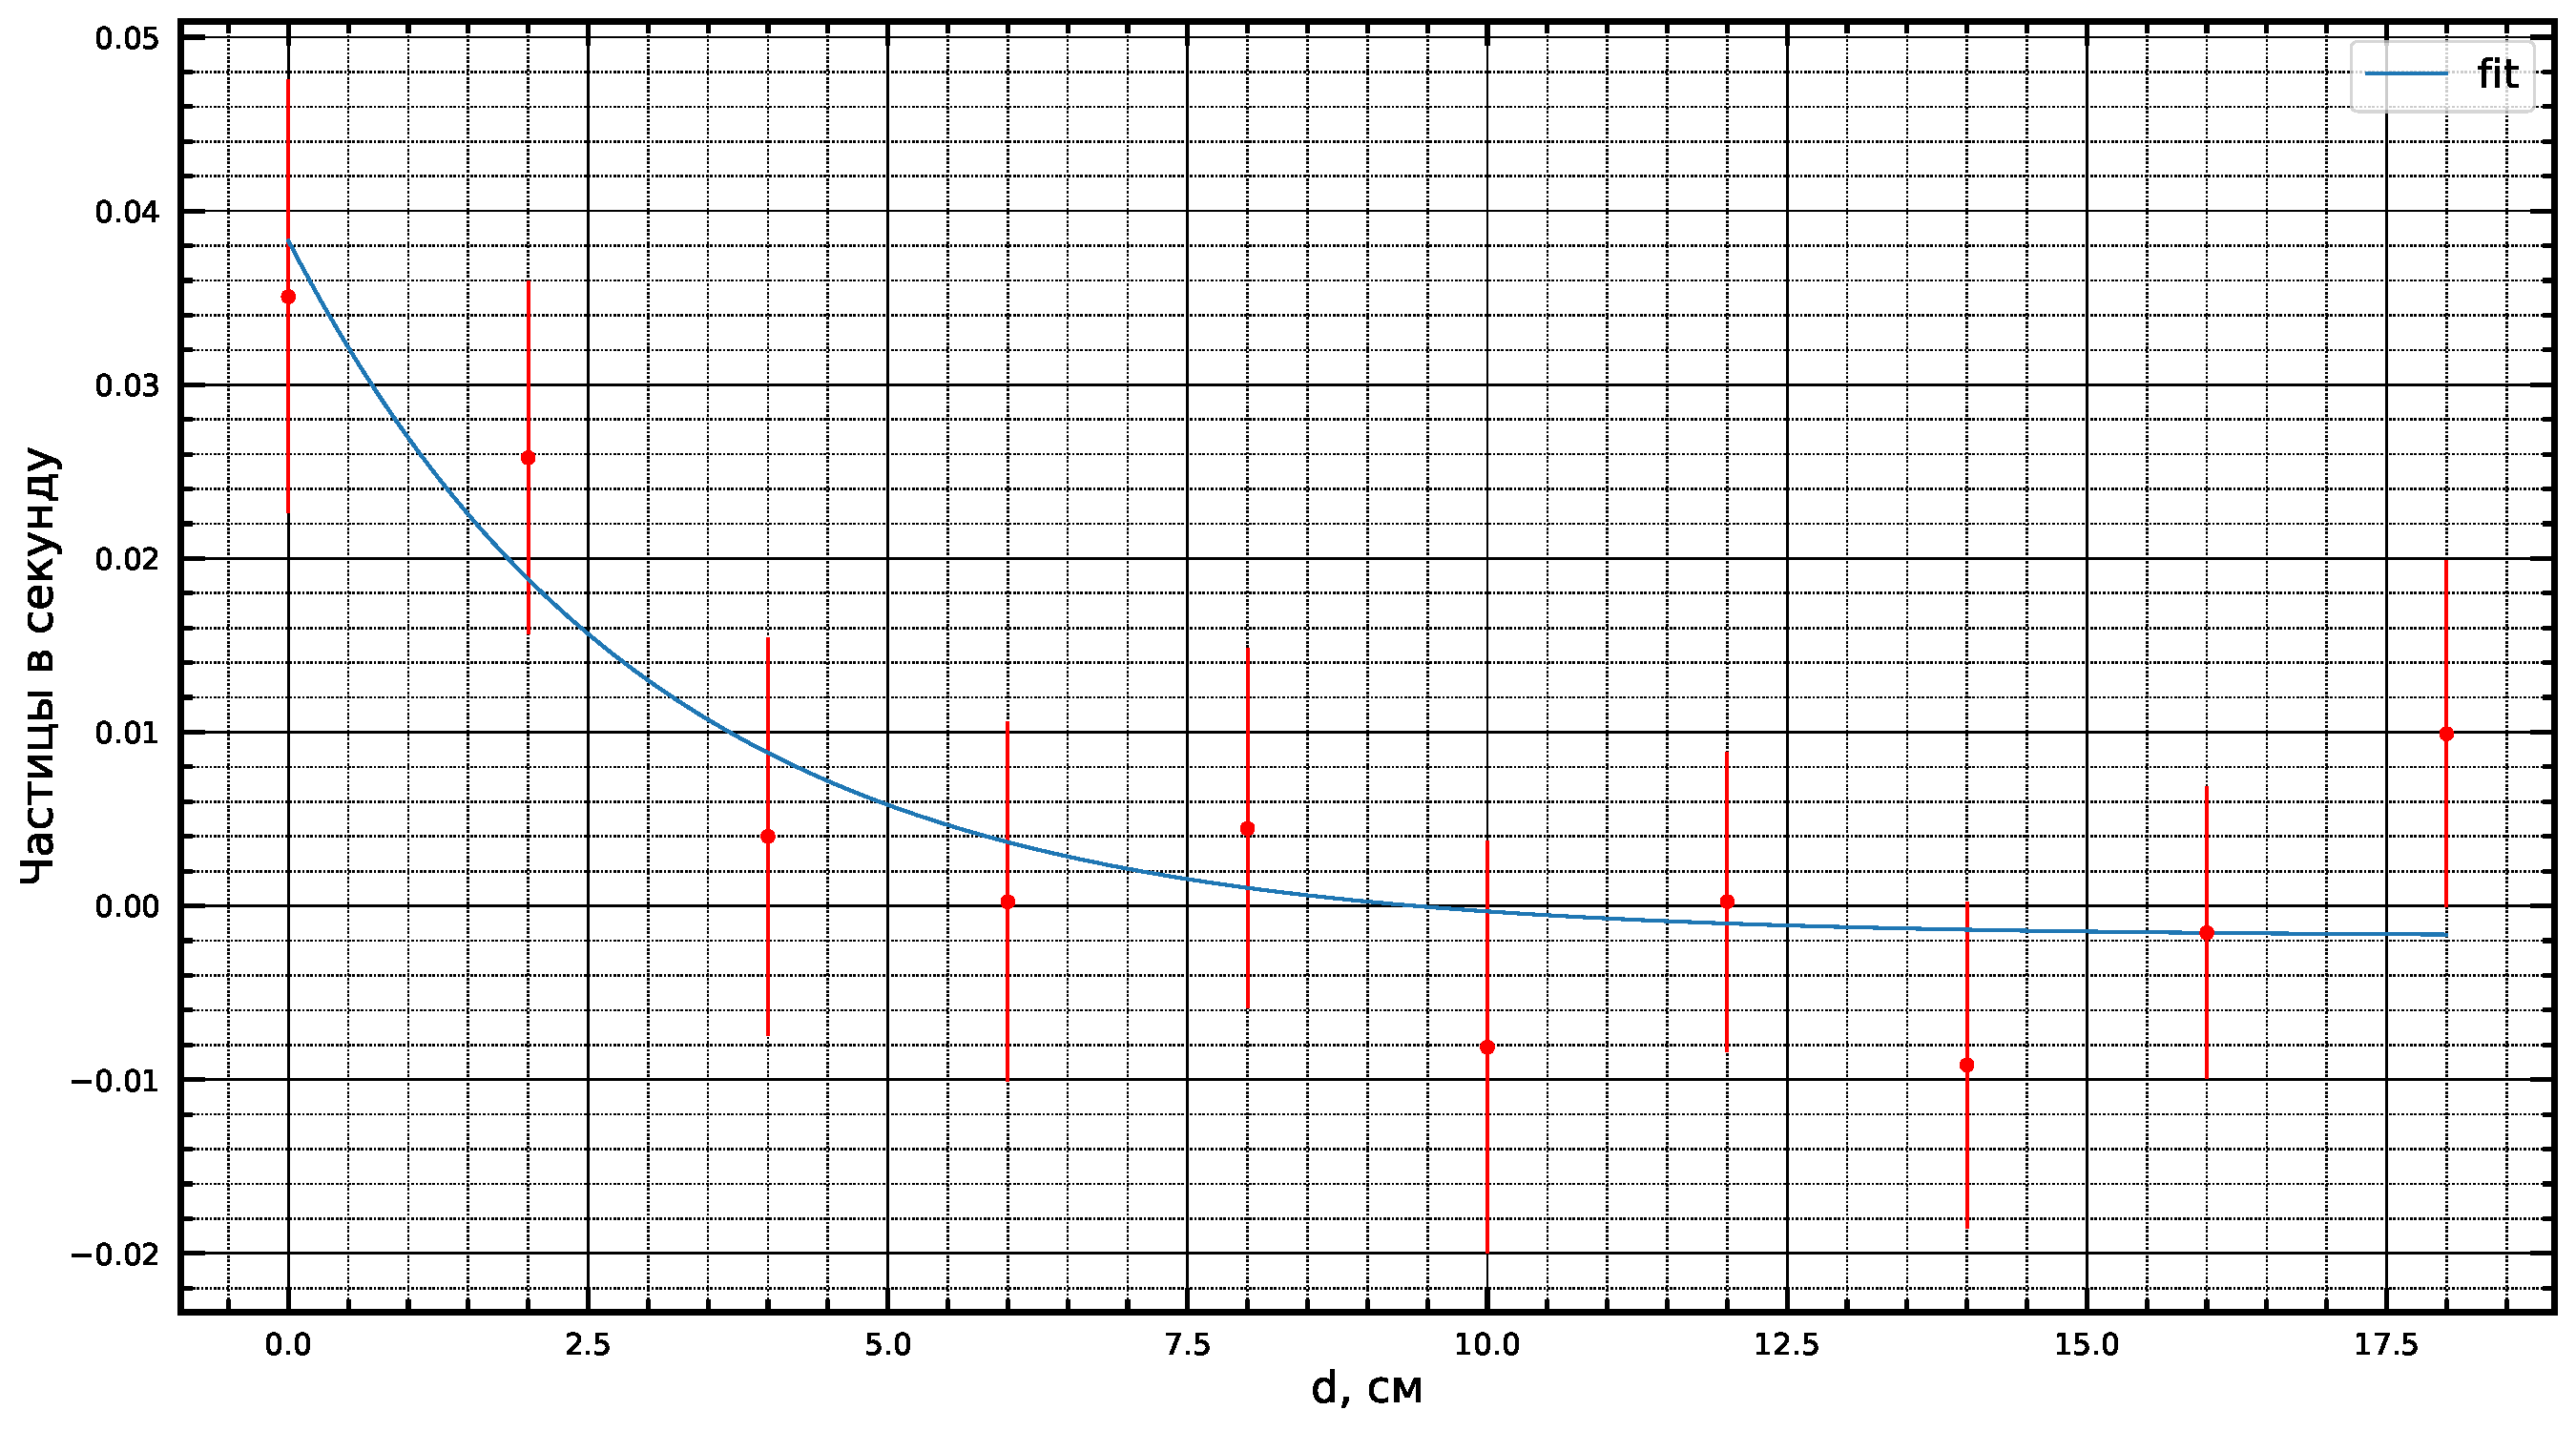
\includegraphics[width=0.95\linewidth]{plot_2.pdf}
	\caption{Зависимость количества частиц мягкой компоненты от толщины поглотителя}
	\label{graph:soft}
\end{figure}

\begin{figure}[h!]
	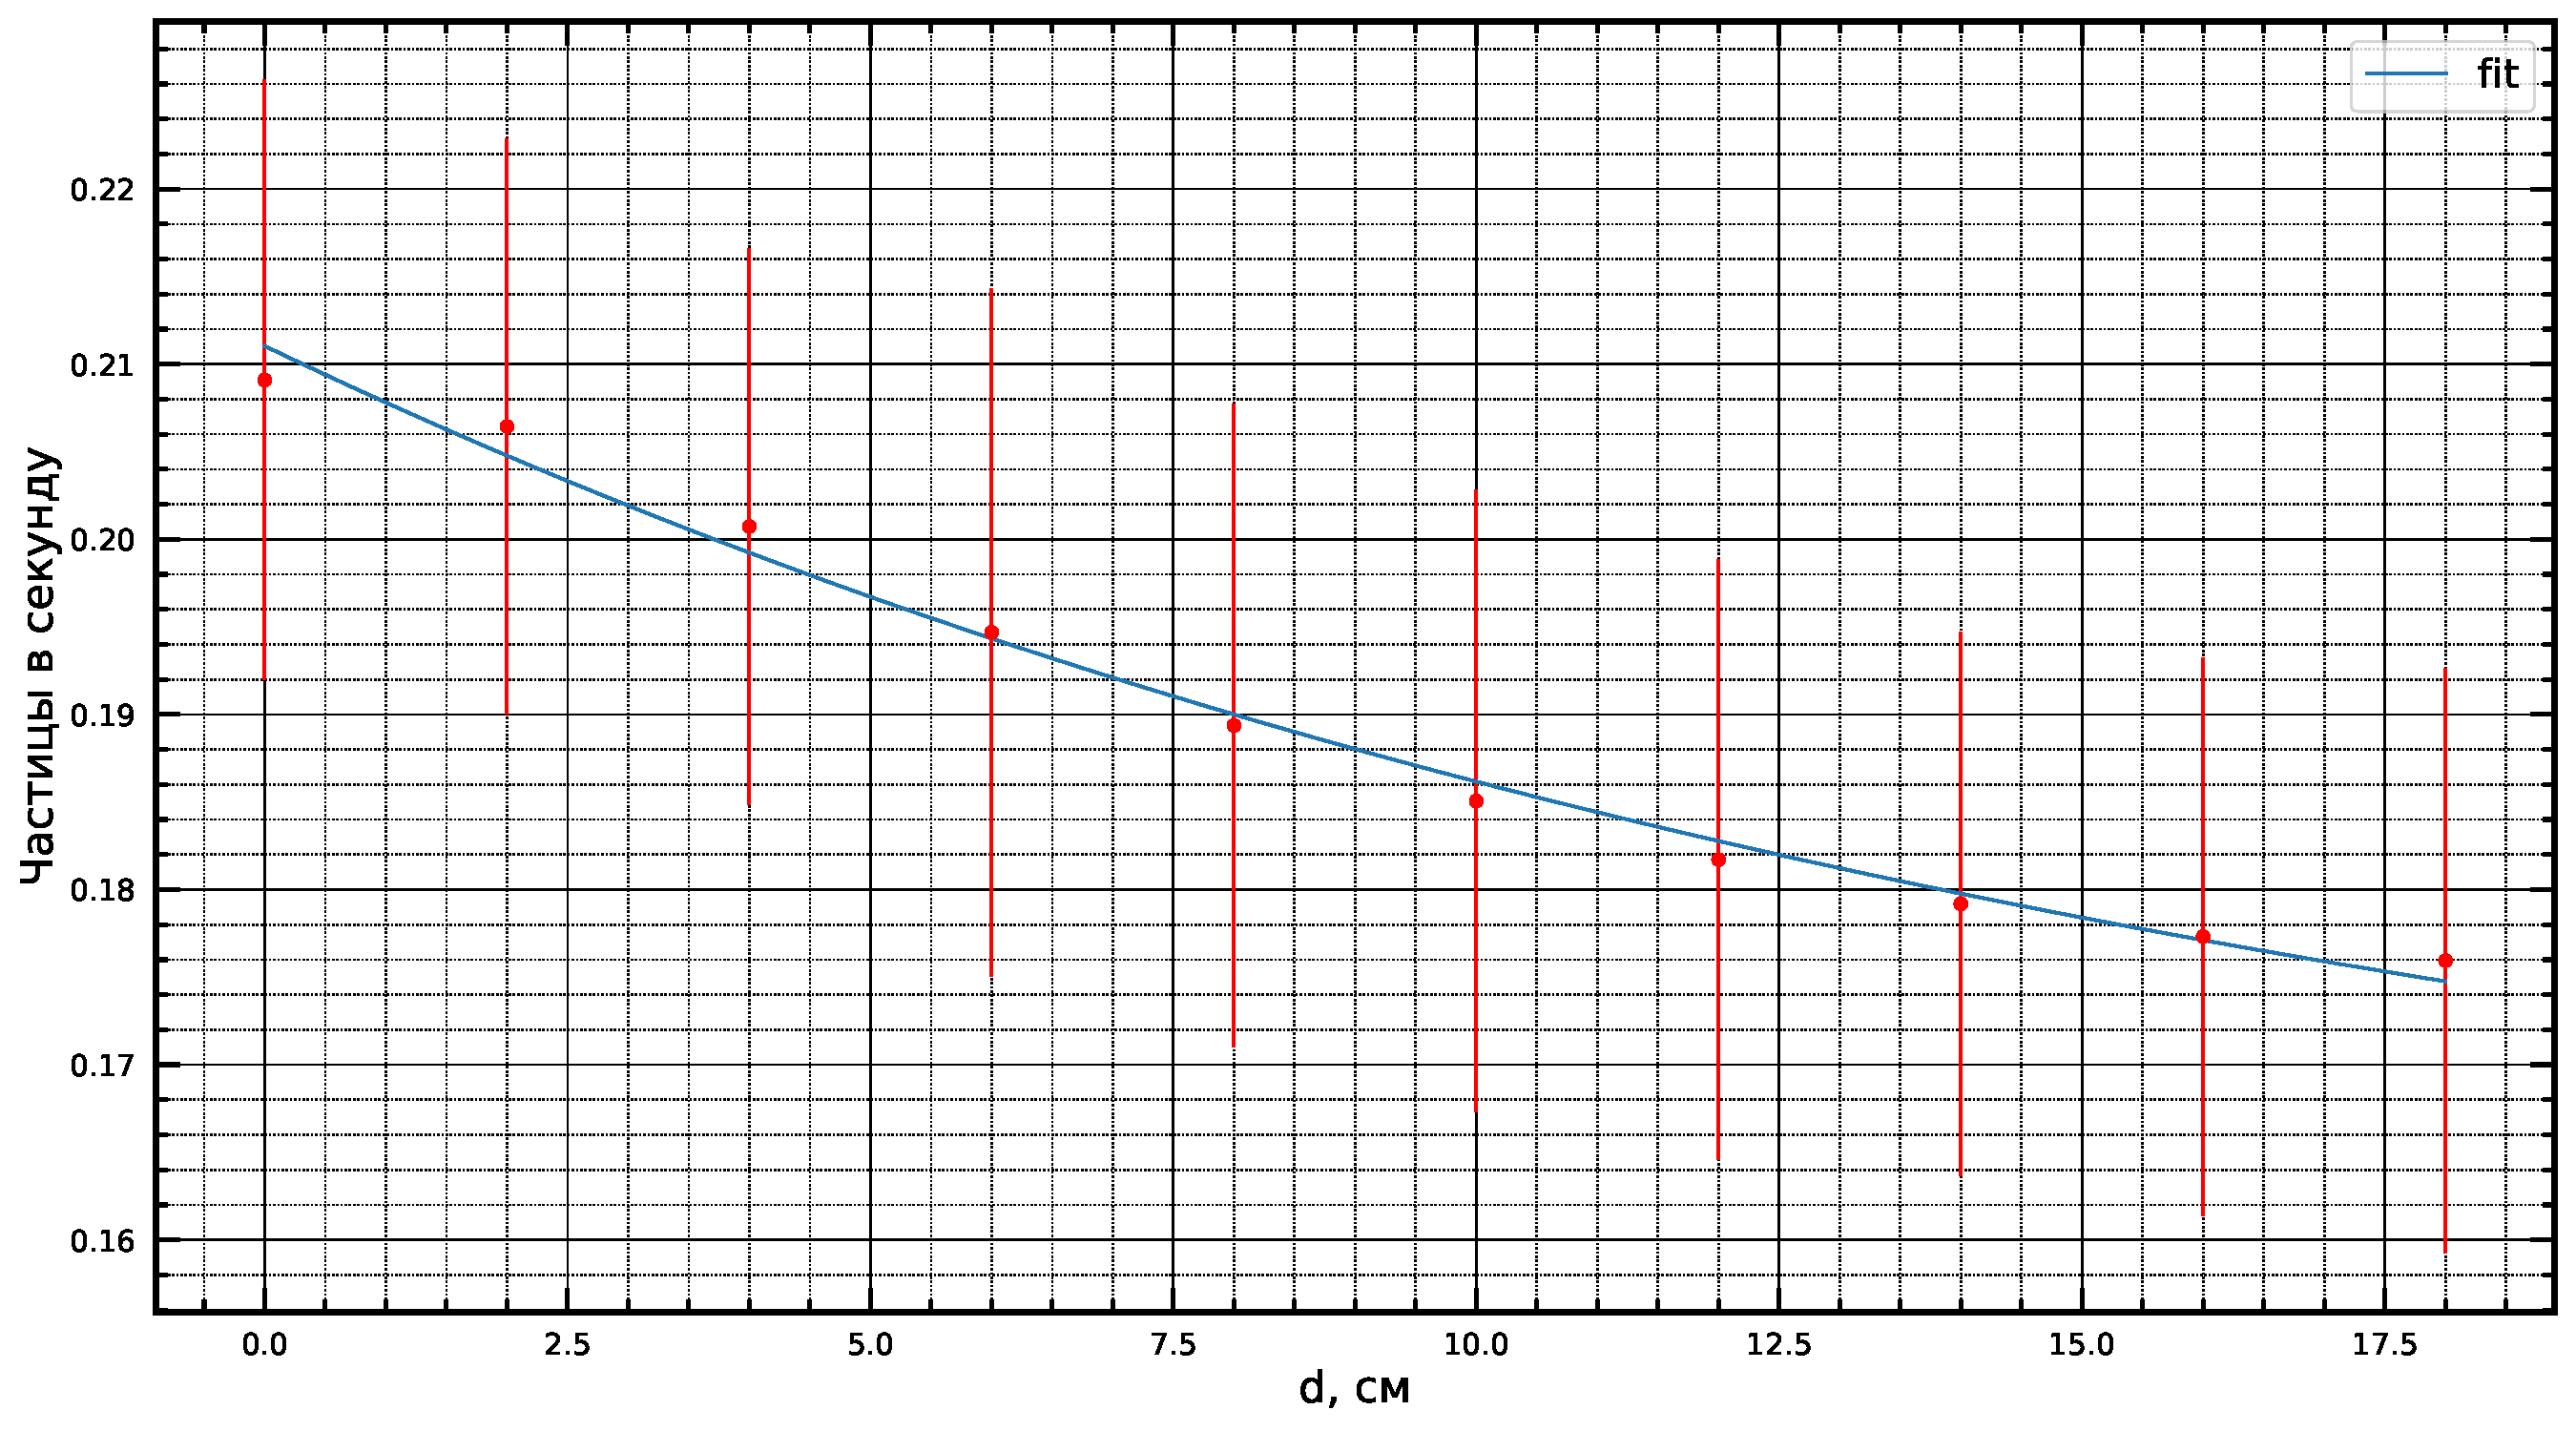
\includegraphics[width=0.95\linewidth]{plot_3.pdf}
	\caption{Зависимость количества частиц жесткой компоненты от толщины поглотителя}
	\label{graph:hard}
\end{figure}

\begin{eqnarray*}
	\lambda_0 &=& 5.93 \cdot 11.34 \approx 67.2 \pm 17.6 \dfrac{\text{г}}{\text{см}^2}\\
	\lambda_{soft} &=& 3.01 \cdot 11.34 \approx 34.1 \pm 15.9 \dfrac{\text{г}}{\text{см}^2}\\
	\lambda_{hard} &=& 16.33 \cdot 11.34 \approx 185.2 \pm 48.6 \dfrac{\text{г}}{\text{см}^2}
\end{eqnarray*}

\newpage
Также рассчитаем телесный угол, из которого регистрируются частицы вторичного излучения.
И после этого интенсивности мягкой и жесткой компонент:


\begin{eqnarray*}
	\Omega &=& \dfrac{4 \cdot 8.4 \cdot 30}{39^2} = 0.66 \pm 0.03 \text{ стер} \\
	I_{soft} &=& \dfrac{N_{soft}}{S \Omega t} = 21 \pm 8 \cdot 10^{-5}
		\dfrac{\text{частиц}}{\text{см}^2 \cdot \text{стер} \cdot \text{с}} \\
	I_{hard} &=& \dfrac{N_{hard}}{S \Omega t} = 125 \pm 7 \cdot 10^{-5}
		\dfrac{\text{частиц}}{\text{см}^2 \cdot \text{стер} \cdot \text{с}} \\
\end{eqnarray*}


\section*{Вывод}

В ходе данной работы были измерены эффективные длины пробега для вторичного космического
излучения и для его мягкой и жесткой компонент в частности. В связи с ограниченным
временем проведения эксперимента, результаты получились неточными (относительная
погрешность для $\lambda_{hard} \approx$~46\%, а для $\lambda_0$ и
$\lambda_{soft} \approx$~24\%). Большая погрешность $\lambda_{hard}$ может быть
обусловлена отсутствием достаточного количества поглотителя, используемого в эксперименте,
что привело к использованию косвенного метода вычисления.

Также были рассчитаны интенсивности мягкой и жесткой компонент (относительные погрешности этих
величин составляют 36\% и 6\% соответственно). Погрешность интенсивности мягкой компоненты
заметно больше чем жесткой. Это связано с тем, что количество частиц мягкой компоненты,
зарегистрированное в эксперименте, значительно меньше общего числа частиц, в чем можно
убедится из графиков (рис.~\ref{graph:gnrl},~рис.~\ref{graph:soft})

\newpage
\appendix

\section*{Таблицы}

\begin{table}
\centering
\caption{Данные с первой установки}
\label{tab:data1}
\begin{tabular}{rcrcc}
\toprule
 $t$, с & \hspace*{10pt} &  $N$, шт & \hspace*{10pt} &  $N_{\text{пласт}}$, шт \\
\midrule
  720 & & 153 & & 1 \\
  720 & & 152 & & 2 \\
  720 & & 146 & & 3 \\
  720 & & 139 & & 4 \\
  720 & & 129 & & 5 \\
  720 & & 118 & & 6 \\
  720 & & 127 & & 7 \\
  720 & & 146 & & 8 \\
  720 & & 125 & & 9 \\
  720 & & 128 & & 7 \\
  720 & & 125 & & 8 \\
  720 & & 179 & & 0 \\
  720 & & 125 & & 6 \\
  720 & & 177 & & 1 \\
\bottomrule
\end{tabular}
\end{table}

\begin{table}[h!]
\centering
\caption{Данные со второй установки}
\label{tab:data2}
\begin{tabular}{rcrcc}
\toprule
 $t$, с & \hspace*{10pt} &  $N$, шт & \hspace*{10pt} &  $N_{\text{пласт}}$, шт \\
\midrule
  900 && 216 && 0 \\
  900 && 209 && 1 \\
  900 && 179 && 2 \\
  600 && 127 && 3 \\
  600 && 104 && 3 \\
  600 && 117 && 4 \\
  600 && 121 && 4 \\
  600 && 108 && 5 \\
  600 && 124 && 6 \\
  600 && 92  && 7 \\
  600 && 87  && 8 \\
  600 && 116 && 9 \\
  600 && 106 && 9 \\
  600 && 100 && 8 \\
  600 && 118 && 6 \\
\bottomrule
\end{tabular}
\end{table}



\end{document}